\chapter{General Introduction}

\section{The ocean, phytoplankton and why it matters}
The complexity of the ocean and its vast ecosystems has fascinated scientists to this day and most likely will continue to do so far into the future. Myriad life forms are embedded in a matrix so far removed from our mostly dry existence on top the earth’s crust. In the ocean, life moves in dilution, and the equivalents of forests and grasslands are hard to spot unless the concentration of tiny phytoplankton is so large, that deep blue turns into a milky green.

The term phytoplankton refers to microscopic marine photosynthetic organisms. These microorganisms form the basis of the oceanic food web and are primary producers of planetary scale, contributing roughly half of the oxygen in our atmosphere through photosynthesis \citep{Field2009}. Phytoplankton consists of mostly single-celled organisms, prokaryotes and eukaryotes from a highly diverse evolutionary background \citep{Falkowski2004a}. This large genetic diversity is accompanied by a remarkable range of survival strategies, biogeochemical roles, shapes and sizes within the polyphyletic phytoplankton (see Figure \ref{FinkelPhySizeRange} for a size comparison).

\begin{figure}
\centering
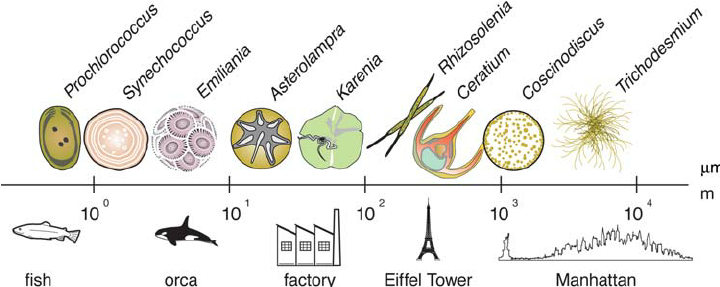
\includegraphics[trim = 0mm 0mm 0mm 0mm, clip, width=.9\linewidth]{./Chp1-Intro/SIZEphytoComparison_FinkelEtAl2010.png}
\caption[Scheme]{\small {"A comparison of the size range (maximum linear dimension) of phytoplankton
relative to macroscopic objects." from \cite{Finkel2010}}}
\label{FinkelPhySizeRange}
\end{figure}

The distribution of phytoplankton is driven by the complex physical forces that govern ocean currents and the chemistry of the bodies of water the move. The key components are macronutrients (e.g. nitrogen \& phosphorus) and micronutrients (e.g. iron \& cobalt) welling up from the deeper ocean or flushed in from continental sources. Wherever there are sufficient nutrients available within the euphotic zone, the depth where photosyntheticaly available radiation (PAR) is 1\% of the surface value, planktonic life begins to thrive. Ecosystems along continental margins provide a particularly productive habitat, with only 10\% of total ocean surface area covered by continental margins, but 10-15\% of marine primary production and more than 40\% of carbon export to the seabed occurring along coastal lines \citep{Yool2001,Muller-Karger2005}.


Phytoplankton growth indirectly feeds a considerable part of earth’s population through fisheries \citep{Stock2017} and even shapes the elemental composition of oceanic water itself \citep{Redfield1958}. 
The biomass produced is mostly consumed by higher trophic levels and either assimilated or excreted. Another large portion experiences natural mortality and viral lysis. Microbial degradation drives remineralization within the euphotic zone, which fuels regenerated production \citep{Eppley1979} [Perhaps put quotation about Microbial Loop here!]. 
A small fraction sinks out of the photic layer as fecal or detrital matter to the deeper ocean and an even smaller fraction reaches the sea floor as sediment ( 1 \%) and remains there over geological times \citep{Honjo2008}. This process has been termed the biological carbon pump. Carbon sequestered this way is removed from the ocean-atmosphere system for potentially millions of years. Given the projected rise of atmospheric CO$_2$ levels, it is of grave importance to understand how changes in the phytoplankton community at the surface, driven by anthropogenic stressors and climate change, will affect the carbon burial potential of oceanic ecosystems. 
Studies have both reported a global declining trend in marine primary production \citep{Boyce2012} and increasing trends in long-term ocean time series \citep{Chavez2011a}. 
In order to answer questions of how phytoplankton will respond to a changing climate it is necessary to look the diverse phytoplankton community in greater detail. 

\section{Characterizing phytoplankton}

Given the relevance of phytoplankton to the global 

How did Researchers start dealing with Phytoplankton?

Two approaches to isolate strains, or take bulk properties

Obviously bulk properties also have to be taken from specific depth

so this adds the problem of the complexity of the physical environment that is the ocean, with enormous volume, turbulunce mixing, diffusion and absorbance

I want to look at phytoplankton diversity, particularly from a functional type point of view. Quantify diversity as it relates to ecosystem function (as production for example).

The emergence of such a large range of organisms and the mechanisms sustaining their persistence has been one of the key topics in phytoplankton ecology over the last 50 years. Hutchinson's paradox.

"Moreover, major taxonomic groups of eukaryotic phyto- plankton can be classified into distinct functional groups (Iglesias-Rodriguez et al. 2002a) with unique biogeochemical signatures. Here, we combine the trait-based approach with the taxonomic sLASh phylogenetic information by broadly sam- pling relevant traits across major taxonomic groups of marine phytoplankton to gain new insights into the effects of evolutionary history on the physiological trait distribu- tions and community structure. An important aspect of a trait-based approach to
"community ecology is the trade-offs between traits (Tilman 1990; Grover 1991; Bohannan et al. 2002). When compe- tition for multiple resources is considered, species are thought to have trade-offs in their competitive ability for one vs. another nutrient (Tilman 1982) or for nutrient vs. light (Huisman \& Weissing 1994; Leibold 1997; Klausmeier \& Litchman 2001). Under non-equilibrium conditions, a trade-off between competitive ability and maximum growth rate may
Litchman, E., Klausmeier, C. A., Schofield, O. M., \& Falkowski, P. G. (2007). The role of functional traits and trade-offs in structuring phytoplankton communities: Scaling from cellular to ecosystem level. Ecology Letters, 10(12), 1170–1181. https:doi.org10.1111j.1461-0248.2007.01117.x


"Functional types can be composed of a large number of species with very different trait values, so the representation of a type by an average trait value may not be appropriate." (Irwin and Finkel 2018)
XXX

"Phytoplankton can be characterised by many morphological, physiological, behavioural and life history traits and trade-offs \citep{Litchman2008, Litchman2010}.

"Studies on the phytoplankton community composition and their response to the environmental gradients are not novel. Ramón Margalef was probably one of the first ecologist to give an important momentum to the topic.  \citep{Margalef1978} used observations of key traits, such as nutrient utilization and sinking rates, to support his well known concept called "Margalef's mandala". His classification of phytoplankton functional types (PFTs) at different nutrient and turbulent environmental conditions represents an excellent first example of how the trait-based notion can be applied to better understand phytoplankton community ecology, therefore setting up the stage for further developments in the field.


\subsection{Functional types and traits}

“Ecology has traditionally focused on species diversity as a way of characterizing the
health of an ecosystem. In recent years, however, the focus has increasingly shifted
towards trait diversity both within and across species” - from Functional Diversity Book

We have incredibly diverse Phytoplankton, and want to analyze traits and model -> need to simplify somehow => Functional Types

so I want to talk about:
that phytoplankton can be divided in functional groups
talk about the Work that Finkel and Irwin have done! 
question whether it makes sense to use functional types instead of species, …
Thus, photopigment-based measures offer an efficient way to quantify community or functional diversity (X Moreno et al., 2012 X). (From Pinckney et al 2015)



XXXX


XXXX


XXXX


\section{Modeling phytoplankton communities}
Going into the details is necessary to understand the whole picture

One tool of integration are mathematical models

Given the complexity of the ocean ecosystem, it is necessary to aggregate our knowledge of the many smaller parts into comprehensive ecological models in order to understand the full-scale implications. 

Computational models of phytoplankton growth have been developed since the 1970s and have greatly increased in sophistication and complexity since then, co-evolving with the rise in computational resources. Ecosystem modelling started with simple box-model descriptions of a few trophic levels. These were the nutrient-phytoplankton-zooplankton (NPZ) and nutrient-phytoplankton-zooplankton-detritus (NPZD) models, which succeeded in reproducing the basic bloom dynamics observed in the temperate ocean (Evans 1988, Fasham et al. 1990). However, in their generalistic approach, these models unavoidably limit the characterization of a diverse phytoplankton community (Bruggeman 2009). To make up for this shortcoming, in the following two decades, these models were expanded to more complex plankton functional type (PFT) models (Le Quere et al. 2005). 

For every group of species that fulfill a distinct ecosystem function, a new set of parameters was added, complicating the model structure and massively prolonging calculations. This somewhat intuitive approach of having every functional group represented in a model, however, did create problems. First and foremost, this is the lack and inherent uncertainty of data from field and culture experiments to constrain functional types. 

This again leads to the difficulty of validating the model output in light of insufficient information (Shimoda et al. 2016 ).Trait-based modeling, on the other side, tries to circumvent the problem of biodiversity (i.e. complexity) in natural systems with a radically different approach. The interactions of phytoplankton with their environment are based on multiple traits which characterize generalized physiological properties like nutrient affinities or motility. Ideally, these traits can be directly measured and are independent of species and therefore they can be directly related to the properties of the organisms function within the ecosystem, such as nutrient affinity for example deally, these traits can be directly measured and are independent of species and therefore they can be directly related to the properties of the organisms function within the ecosystem, such as nutrient affinity for example (Litchman and Klausmeier 2008).  


A simple example of a trait-based description of phytoplankton succession is scaling the maximal nutrient acquisition rate and the respective affinity with cell size. A trade-off would emerge between different size classes, allowing for a modeled succession along gradients of nutrient depletion. One example of a very similar approach is the PhytoSFDM model developed by Acevedo-Trejos and colleagues (Acevedo‐Trejos et al. 2013, Acevedo-Trejos et al. 2015). In their approach, the trait-based modelling of phytoplankton is even further simplified, by describing an entire community as a size- distribution with a mean value and a variance, instead of modeling all the different size classes explicitly. This moment-based structure further simplifies the mathematical basis of the model, and leads to much faster processing times and less uncertainty in parameter estimation.



"quite a few publications using models go too far in their extrapolations, whilst the general discussion still strongly revolves around meaningful model structures.. but no consensus is anywhere to be seen!
"need to identify the basic uncertainties and see if there is a way to discuss them scientifically
"Michaelis Menten kinetics are really outdated.. and i suppose using them in a trait-based modelling approach is questionable just the same
"plankton ecosystems are typically highly aggregated, a single variable gives the response of an incredibly diverse assemblage of phytoplankton species (P. Franks, 2009)


\begin{figure}
\centering
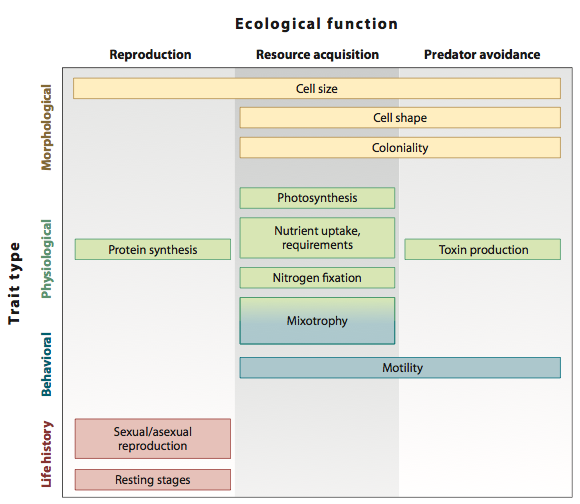
\includegraphics[width=0.7\linewidth]{./Chp1-Intro/Fig_litchman2008.png}
\caption[Scheme]{\small{Phytoplankton functional traits. Taken from \citet{Litchman2008}}}
\label{phytotrait}
\end{figure}

XXX

XXX

XXX

XXX. 

XXX

XXX

ALWAYS NEED A GOOD BASIS IN DATA TO VALIDATE MODELS AND HYPOTHESES

\section{The Cariaco basin \& the CARIACO time series}

A coastal tropical ecosystem

"continental margins constitute only about 10\% of the total ocean surface area, these regions are responsible for about 10–15\% of the global marine primary production and greater than 40\% of seabed carbon sequestration (Yool and Fasham, 2001; Muller-Karger et al., 2005). 
"The Cariaco Basin, located off the coast of Venezuela, has been the site of high frequency water column sampling for marine biogeochemical and ecological observations since 1995. The observations were collected as part of the Cariaco Ocean Time-Series Program (Muller-Karger et al., 2001; Thunell et al., 2007). 

XXXX

In addition to the recent importance of the cariaco basin as the site of an important paleo-oceanographic time sereis, the Cariaco basin has served as a natureal laboratory for biogeochemists for over 50 years. This basin has been key in constructiong stoichiometric models of organic matter remineralization (Redfield et al 1963 and Richards 1975!), developing residence time and box models, and numerous other studies.

\begin{figure}
\centering
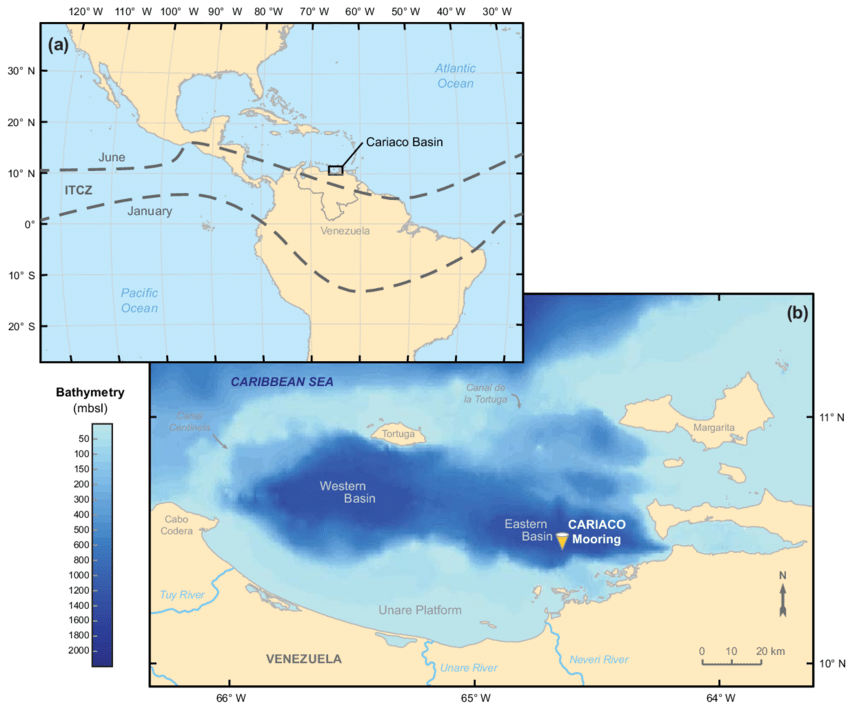
\includegraphics[trim = 0mm 0mm 0mm 0mm, clip, width=1.\linewidth]{./Chp1-Intro/CARIACObasinMAP_Bringueetal2018.png}
\caption[Scheme]{\small {"Study area. A. Location of the Cariaco Basin off the Venezuelan coast in the southern Caribbean Sea, with January and June positions of the Intertropical Convergence Zone (ITCZ). B. Location of the CARIACO station in the eastern sub-basin, general bathymetry and local rivers emptying in the basin (bathymetric data from GEBCO\_08 Grid)" from \cite{Bringue2019}}}
\label{CARIACO-map}
\end{figure}

XXXX

XXX

THEN TALK ABOUT THE COLLABorDATASHARE WITH JPINCKNEY AND CBENITEZNELSON, and how this allows an even deeper look at the biomass dynamics


\section{Aims of the proposed PhD project}
"The general goal of my Ph.D. project is to study the processes that structure the phytoplankton community in contrasting environmental regions of the Atlantic Ocean, using a trait-based modelling perspective. The specific aims during the course of the project are to:

\begin{itemize}
\item MANUSCRIPT 1 "Understanding Shifts in CARIACO"
\item MANUSCRIPT 2 "technical paper" - Geoscientific Model development
\item MANUSCRIPT 3 "BDEF in CARIACO"
\end{itemize}
